%%% PREAMBLE - Do not touch %%%%%%%%%%%%%%%%%%%%%%%%%%%%%%%%%%%%%%%%%%%%%%%%%%%%%%
\documentclass[10pt,twocolumn,letterpaper]{article}
\usepackage[utf8]{inputenc}
\usepackage[portuges,brazil,english]{babel}
\usepackage{model}
\usepackage{times}
\usepackage{epsfig}
\usepackage{graphicx}
\usepackage{amsmath}
\usepackage{amssymb}
\usepackage{color}
\usepackage[pagebackref=true,breaklinks=true,letterpaper=true,colorlinks,bookmarks=false]{hyperref}

\cvprfinalcopy % *** Uncomment this line for the final submission
\def\httilde{\mbox{\tt\raisebox{-.5ex}{\symbol{126}}}}
\ifcvprfinal\pagestyle{empty}\fi

\newcommand{\TODO}[1]{TODO: #1}
\newcommand{\CITEONE}[2]{\mbox{#1 \cite{#2}}}
\newcommand{\CITETWO}[3]{\mbox{#1 and #2 \cite{#3}}}
\newcommand{\CITEN}[2]{\mbox{#1 et al. \cite{#2}}}

%%% Paper beginning %%%%%%%%%%%%%%%%%%%%%%%%%%%%%%%%%%%%%%%%%%%%%%%%%%%%%%%%%%%%%%
\begin{document}

%%% Title and authors %%%%%%%%%%%%%%%%%%%%%%%%%%%%%%%%%%%%%%%%%%%%%%%%%%%%%%%%%%%%
\title{MC886 - Trabalho prático 2}
\author{Guilherme P. Gonçalves (RA 091429)}

%%% Abstract %%%%%%%%%%%%%%%%%%%%%%%%%%%%%%%%%%%%%%%%%%%%%%%%%%%%%%%%%%%%%%%%%%%%%
\maketitle
\begin{abstract}
Este trabalho explorou técnicas de redução de dimensionalidade no contexto de uma aplicação de reconhecimento de faces. Diversas variações de um algoritmo de reconhecimento de faces utilizando Principal Component Analysis e Linear Discriminant Analysis foram implementadas e testadas sobre um conjunto de aproximadamente 3 mil fotografias de pessoas.
\end{abstract}

%%% Introduction %%%%%%%%%%%%%%%%%%%%%%%%%%%%%%%%%%%%%%%%%%%%%%%%%%%%%%%%%%%%%%%%%
\section{Introdução}

Algoritmos de redução de dimensionalidade são fundamentais em diversas aplicações de aprendizado de máquina tanto para reduzir a complexidade de um modelo, tornando-o computacionalmente mais barato, quanto para melhorar a separabilidade dos dados em problemas de classificação, melhorando assim a qualidade da aplicação.

Neste trabalho, foram explorados os usos de duas técnicas de redução de dimensionalidade, Principal Component Analysis (PCA) e Linear Discriminant Analysis (LDA), a um problema de reconhecimento de faces em que os dados de treinamento e teste eram imagens de pessoas cujos pixels deveriam ser utilizados como \emph{feature vectors}.

A Seção \ref{sec-problem} descreve em mais detalhes a proposta deste trabalho, enquanto a Seção \ref{sec-algorithm} descreve algumas particularidades dos algoritmos desenvolvidos e de suas implementações. A Seção \ref{sec-experiments} contém os resultados experimentais da aplicação dos algoritmos a um conjunto de imagens de faces.

\section{O problema analisado}
\label{sec-problem}

O problema analisado neste estudo é uma aplicação clássica da área de aprendizado de máquina: o reconhecimento de faces. Especificamente, dado um conjunto de 3414 fotografias de pessoas em tons de cinza, dividido em um grupo de "referência" de 3214 imagens e outro de "consulta" contendo 200 imagens, construiu-se de diversas formas um banco de dados de referência (BDR) a partir do primeiro grupo, e um banco de dados de consulta (BDC) a partir do segundo. Avaliou-se então o efeito das diferentes formas de construir tais bancos de dados sobre o número de classificações corretas das imagens em BDC usando BDR para as consultas.

Como restrição prévia, todas as imagens deveriam ser associadas a \emph{feature vectors} dados pelos valores de seus pixels linearizados em ordem de linhas. Ou seja, para uma imagem de 50x50 pixels, o \emph{feature vector} deveria ter dimensão 2500, sendo que as primeiras 50 dimensões seriam os valores dos pixels na primeira linha da matriz da imagem. O uso de \emph{feature vectors} grandes sugere a aplicação de técnicas de redução de dimensionalidade, que foram o grande objeto de análise neste trabalho.

\section{Descrição dos algoritmos}
\label{sec-algorithm}

Todos os algoritmos implementados para este trabalho eram variantes de um método geral, que consiste em computar os \emph{feature vectors} a partir das imagens e, para cada imagem em BDC, encontrar a imagem mais próxima a ela no BDR e usar a pessoa correspondente a ela como resultado da classificação. Sobre essa ideia geral foram variados os métodos de construção de \emph{feature vectors} e de cálculo de distância entre eles.

Uma mesma etapa de pré-processamento das imagens precedeu a aplicação de todos os algoritmos, visando a tornar as imagens mais representativas das pessoas retratadas. Para cada uma das imagens conheciam-se as posições dos centros dos dois olhos, do nariz e da boca. A etapa de pré-processamento usava essas informações para produzir uma imagem de tamnho reduzido (o mesmo tamanho para todas as imagens) que tentasse capturar a maior parte da face representada.

A técnica de recorte do rosto utiliza proporções simples comumente aplicadas por ilustradores ao desenhar rostos humanos \cite{FacialProportions:2010:Online}. Por exemplo, a distância entre os cantos internos dos olhos é aproximadamente igual à largura de um olho, e a largura da face é próxima de cinco vezes essa largura. Utilizando essas aproximações e as coordenadas disponíveis, cada imagem tem seu rosto recortado e é redimensionada para um tamanho comum. A Figura \ref{fig-cropping} apresenta uma imagem original (reduzida para ilustração apenas) à esquerda, e sua versão pré-processada em tamanho 50x50 à direita. Na seção \ref{sec-experiments} foram testados diferentes tamanhos de imagens pré-processadas.

\begin{figure}
\begin{center}
	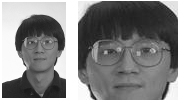
\includegraphics[width=0.99\columnwidth]{pics/cropping.png}
	\caption{Imagem original (esq.) e pré-processada (dir.), após o recorte da face e redimensionamento para 50x50.}
	\label{fig-cropping}   
\end{center} 
\end{figure}  

Os algoritmos testados operam a seguir sobre essas imagens pré-processadas. Esses algoritmos são denominados \emph{plain}, \emph{pca}, \emph{lda}, \emph{pca.lda} e \emph{lda.pca}.

O algoritmo \emph{plain} considera como \emph{feature vectors} as imagens inteiras, com cada dimensão dada pelo valor do pixel correspondente (normalizado pelo valor máximo de 255, ou seja, variando no intervalo de 0 a 1).

Os algoritmos \emph{pca} e \emph{lda} usam PCA e LDA sobre os \emph{feature vectors} do algoritmo \emph{plain}. Especificamente, as técnicas de redução de dimensionalidade são aplicadas aos vetores em BDR para encontrar uma transformação com dimensionalidade reduzida; essa transformação era depois aplicada ao BDC antes das consultas. Para o algoritmo LDA, foi utilizada como classe a pessoa retratada na foto. Os algoritmos \emph{pca(lda)} e \emph{lda(pca)} usam PCA sobre os resultados do LDA e LDA sobre os resultados do PCA, respectivamente.

Uma vez calculados os  \emph{feature vectors} para cada imagem do BDR e BDC, as imagens do BDC são classificadas utilizando a imagem com vetor mais próximo no BDR, dado, para todos os algoritmos acima, pela distância Euclidiana. Também foram conduzidos, na seção \ref{sec-experiments}, experimentos usando norma L-1 da diferença entre os vetores.

Cabe, finalmente, notar alguns aspectos da implementação dos algoritmos, feita inteiramente em R.

Para atingir maior eficiência, a cada consulta a busca pelo vetor mais próximo no BDR foi feita utilizando uma estrutura de dados \emph{k-d} tree encontrada no pacote FNN.

A linguagem R contém duas funções, \emph{princomp} e \emph{prcomp}, para executar o cálculo da PCA. A primeira utiliza autovetores e autovalores para decompor a matriz de covariâncias, enquanto a segunda usa SVD. A função \emph{princomp}, embora seja muito mais rápida, está mais suscetível a erros numéricos e só funciona quando o número de vetores de entrada é maior que o número de dimensões. Como não se observaram diferenças nos resultados finais dos testes ao se utilizar as diferentes funções, as implementações dos algoritmos buscam usar \emph{princomp} quando possível por razões de eficiência, recorrendo a \emph{prcomp} em testes de maior dimensionalidade.

\section{Resultados experimentais}
\label{sec-experiments}

Esta seção contém os resultados experimentais das aplicações dos diferentes algoritmos. Todos os algoritmos mencionados na Seção \ref{sec-algorithm} foram testados variando-se a quantidade de "energia" retida pelo algoritmo PCA (95\% e 99\%) e o tamanho das imagens pré-processadas (50x50, 75x75 e 100x100, além dos tamanhos 64x96 e 32x48, que mantêm o aspecto das imagens originais).

De todas as pessoas com imagens no BDC, apenas uma delas não aparecia também no BDR. Dessa forma, era possível classificar corretamente no máximo 199 das 200 pessoas no BDC. O melhor algoritmo em cada teste foi também avaliado usando como medida de distância entre vetores a norma L-1 em vez da distância Euclidiana.

A Tabela \ref{tbl-95} contém o número de acertos para cada tamanho de imagem e método quando o algoritmo PCA foi configurado para reter 95\% da energia dos vetores das imagens. As colunas referem-se aos algoritmos conforme explicados na Seção \ref{sec-algorithm}. A coluna L-1 contém os resultados de se usar o algoritmo com maior número de acertos (em negrito) adaptado para usar a norma L-1 da diferença entre os vetores como medida de distância. Em caso de empate, foi utilizado o algoritmo mais à esquerda na tabela.

\begin{table*}
\begin{center}
\begin{tabular}{ | l | l | l | l | l | l | l | p{3.5cm} |}
\hline
Dimensão das imagens & plain & pca & lda & lda(pca) & pca(lda) & L-1 \\
\hline
32x48 & 137 & 137 & 93 & \textbf{152} & 93 & 145 \\
64x96 & 136 & 137 & 101 & \textbf{151} & 106 & 141 \\
50x50 & 137 & 137 & 90 & \textbf{149} & 92 & 142 \\
75x75 & 136 & 137 & 102 & \textbf{152} & 107 & 144 \\
100x100 & 136 & 137 & 98 & \textbf{149} & 104 & 138 \\
\hline
\end{tabular}
\end{center}
\caption{Número de acertos para cada método e dimensão de imagens com PCA mantendo 95\% da energia.}
\label{tbl-95}
\end{table*}

A Tabela \ref{tbl-99} é análoga à Tabela \ref{tbl-95}, desta vez com o algoritmo PCA retendo 99\% da energia.

\begin{table*}
\begin{center}
\begin{tabular}{ | l | l | l | l | l | l | l | p{3.5cm} |}
\hline
Dimensão das imagens & plain & pca & lda & lda(pca) & pca(lda) & L-1 \\
\hline
32x48 & 137 & 137 & 93 & \textbf{140} & 93 & 119 \\
64x96 & \textbf{136} & 136 & 101 & 107 & 101 & 147 \\
50x50 & \textbf{137} & 137 & 90 & 128 & 91 & 147 \\
75x75 & \textbf{136} & 136 & 102 & 110 & 102 & 148 \\
100x100 & \textbf{136} & 136 & 98 & 97 & 98 & 149 \\
\hline
\end{tabular}
\end{center}
\caption{Número de acertos para cada método e dimensão de imagens com PCA mantendo 99\% da energia.}
\label{tbl-99}
\end{table*}

Observa-se nas Tabelas \ref{tbl-95} e \ref{tbl-99} que os melhores resultados foram obtidos com a aplicação conjunta dos algoritmos PCA e LDA, nessa ordem, sobre as imagens de entrada, mantendo-se 95\% da informação nas imagens durante a etapa da PCA.

Na Tabela \ref{tbl-95}, em particular, fica evidenciada a utilidade das técnicas de redução de dimensionalidade para tratar o problema, dado que elas proporcionaram uma melhoria de cerca de 10\% sobre o método \emph{plain} quando usadas em conjunto.

Na medida em que a técnica PCA reduz a dimensionalidade dos dados ignorando a informação de classe, não se esperava que ela melhorasse a separabilidade do problema em relação ao método \emph{plain}, o que de fato não ocorreu.

Com 99\% da informação mantida, não se observou melhora tão grande de nenhum método sobre o algoritmo \emph{plain}. De fato, com essa configuração, os maiores números de acertos foram obtidos com a mudança na função de distância sobre os \emph{feature vectors} originais, sem redução alguma de dimensionalidade.

Observa-se ainda que, para uma mesma taxa de retenção de informação, o tamanho das imagens pouco influiu nos resultados finais, sendo imagens menores preferíveis por serem computacionalmente muito mais baratas.

De forma geral obtiveram-se bons resultados de classificação dada a simplicidade dos algoritmos implementados, com taxa de acertos em torno de 75\%  para todos os melhores testes.

\section{Conclusão}

Este trabalho comprovou experimentalmente a utilidade de técnicas de redução de dimensionalidade aplicadas a um problema de reconhecimento de faces.

Foram implementadas diversas variantes de um algoritmo simples evidenciando-se com sucesso a influência da aplicação das técnicas LDA e PCA e obtendo-se resultados razoáveis no reconhecimento em si.

%%% References %%%%%%%%%%%%%%%%%%%%%%%%%%%%%%%%%%%%%%%%%%%%%%%%%%%%%%%%%%%%%%%%%%%
{\small
\bibliographystyle{unsrt}
\bibliography{references}
}

\end{document}
